This analysis highlighted the importance of HTML tags and attributes (image, font, table, width, align, nbsp, size, color, etc.). These terms have high TF-IDF scores, indicating they are highly characteristic and useful for distinguishing between different emails, likely separating HTML-formatted emails from plain text ones.

TF-IDF combines two parts: Term Frequency (TF) and Inverse Document Frequency (IDF).

Term Frequency (TF): Measures how often a word appears in a document.
A higher frequency suggests greater importance.
If a term appears frequently in a document, it is likely relevant to the document’s content.
Formula:
\[
    \text{tf}(t, d) = \frac{f_{t,d}}{\sum_{t' \in d} f_{t',d}}
\]
where $f_{t,d}$ is the raw count of a term $t$ in a document, i.e., the number of times that term $t$ occurs in document $d$.
Note the denominator is simply the total number of terms in document $d$ (counting each occurrence of the same term separately).
There are various other ways to define term frequency:
\begin{itemize}
    \item The raw count itself: $\text{tf}(t,d) = f_{t,d}$
    \item Boolean ``frequencies'': $\text{tf}(t,d) = 1$ if $t$ occurs in $d$ and 0 otherwise;
    \item Logarithmically scaled frequency: $\text{tf}(t,d) = \log (1 + f_{t,d})$;
    \item Augmented frequency, to prevent a bias towards longer documents, e.g., raw frequency divided by the raw frequency of the most frequently occurring term in the document:
\end{itemize}
\[
    \text{tf}(t, d) = 0.5 + 0.5 \cdot \frac{f_{t,d}}{\max\{f_{t',d} : t' \in d\}}
\]

The inverse document frequency (IDF) is a measure of how much information the word provides, i.e., how common or rare it is across all documents.
It is the logarithmically scaled inverse fraction of the documents that contain the word (obtained by dividing the total number of documents by the number of documents containing the term, and then taking the logarithm of that quotient):
\[
    \text{idf}(t, D) = \log \frac{N}{|\{d : d \in D \text{ and } t \in d\}|}
\]

with
\begin{itemize}[leftmargin=2em, itemsep=0.5ex] % Adjust indentation as needed
    \item $N$: Total number of documents in the corpus $N = |D|$
    \item $|\{d \in D : t \in d\}|$: Number of documents where the term $t$ appears (e.g., $\text{tf}(t,d) \neq 0$). If the term is not in the corpus, this will lead to a division-by-zero.
    It is therefore common to adjust the numerator to $1+N$ and denominator to $1 + |\{d \in D : t \in d\}|$.
\end{itemize}

Term frequency--inverse document frequency (TF-IDF):
\[
    \text{tfidf}(t, d, D) = \text{tf}(t, d) \cdot \text{idf}(t, D)
\]

The TF-IDF scores highlight words that are important for distinguishing between different emails in your dataset.
While widespread words like ``the'' have high term frequency, their low inverse document frequency reduces their TF-IDF score because they appear in almost all emails.
Words with higher TF-IDF scores, like ``number' and ``url'' are likely more specific to certain subsets of your email data and could be valuable features for a classification task like spam detection.
The presence of ``you'' also suggests a potential distinction based on the direct address to the recipient.
This visualization helps identify terms that are characteristic of individual emails within the collection.

\begin{figure}[H]
    \centering
    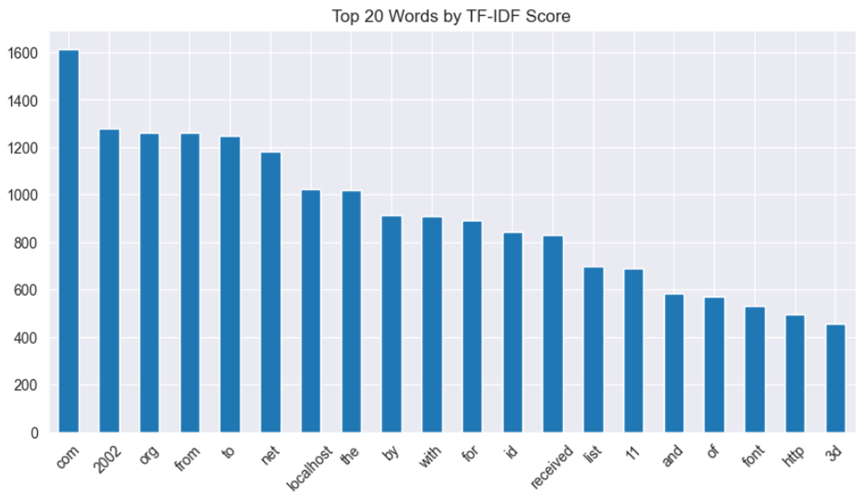
\includegraphics[width=\linewidth]{images/top_tf_idf_score}
    \caption{Bar Chart for Top 20 Words by TF-IDF Score}
    \label{fig:top_tf_idf_score}
\end{figure}

Observations:
\begin{itemize}
    \item ``com'' has the highest TF-IDF score: The word ``com'' has the tallest bar, indicating it has the highest TF-IDF score among the top 20.
    \item ``2002'' and ``org'' have the next highest scores: These words also have relatively high TF-IDF scores.
    \item Words like ``from'', ``to'', ``net'', and ``localhost'' have considerable scores: They suggest some importance in differentiating documents within the corpus.
    \item Common English words have lower scores: Words like ``the'', ``by'', ``with'', ``for'', ``and'', and ``of'' appear in the list but have lower TF-IDF scores compared to the more specific terms.
    This is expected because TF-IDF downweights words that appear frequently across many documents.
    \item Technical terms and identifiers are present: Words like ``id'', ``font'', ``http'', and ``3d'' suggest that these terms might be important in distinguishing certain types of documents within the corpus.
    \item ``received'' and ``list'' also have moderate TF-IDF scores.
    The number ``11'' also appears in the list.
\end{itemize}

Meaning of TF-IDF:
\begin{itemize}
    \item Term Frequency (TF): Measures how frequently a term appears in a document.
    \item Inverse Document Frequency (IDF): Measures how rare a term is across the entire corpus of documents.
    Words that appear in many documents have a lower IDF.
\end{itemize}

A high TF-IDF score for a word means that the word is frequent in a particular document but rare in the overall corpus.
Therefore, these words are considered more important for distinguishing documents.

In summary, this bar chart highlights the words that are most discriminative across the analyzed text documents based on their TF-IDF scores.
The words with higher scores, such as ``com'', ``2002'', ``org'', and ``localhost'', are likely good indicators of the specific content or categories of the documents in which they appear.
The presence of common English words with lower scores confirms the TF-IDF mechanism of prioritizing distinguishing terms.
This analysis is often used in information retrieval and text mining to identify the most relevant terms in a collection of documents.